\documentclass[10pt]{report}
\usepackage[utf8]{inputenc}
\usepackage[italian]{babel}
\usepackage{multicol}
\usepackage[bookmarks]{hyperref}
\usepackage[a4paper, total={18cm, 25cm}]{geometry}
\usepackage{graphicx}
\usepackage{xcolor}
\usepackage{textcomp}
\graphicspath{ {./img/} }
\usepackage{listings}
\usepackage{makecell}
\usepackage{qtree}
\usepackage{pgfplots}
\usepackage{tikz}
\usepgflibrary{shapes}
\usepgfplotslibrary{fillbetween}
\definecolor{backcolour}{RGB}{255,255,255}
\definecolor{codegreen}{RGB}{27,168,11}
\definecolor{codeblue}{RGB}{35,35,205}
\definecolor{codegray}{RGB}{128,128,128}
\definecolor{codepurple}{RGB}{205,35,56}
\lstdefinestyle{myPython}{
	backgroundcolor=\color{backcolour},   
	commentstyle=\color{codegreen},
	keywordstyle=\color{codeblue},
	numberstyle=\tiny\color{codegray},
	stringstyle=\color{codepurple},
	basicstyle=\small\ttfamily,
	breakatwhitespace=false,         
	breaklines=true,                 
	captionpos=b,                    
	keepspaces=true,                 
	numbers=left,                    
	numbersep=2pt,                  
	showspaces=false,                
	showstringspaces=false,
	showtabs=false,                  
	tabsize=2,
	language=python
}
\newcommand*\triangled[1]{\tikz[baseline=(char.base)]{
            \node[regular polygon, regular polygon sides=3,draw,inner sep=1pt] (char) {#1};}}
\begin{document}
\title{Algorithm Engineering}
\author{Federico Matteoni}
\date{A.A. 2021/22}
\renewcommand*\contentsname{Index}

\maketitle
\begin{multicols}{2}
\tableofcontents
\end{multicols}
\pagebreak
\section{Introduction}
Teacher: Paolo Ferragina\\
Exam: written + oral. Midterms in November and December, with exercises.\\
Classes will be recorded on Microsoft Teams. Also the book "The Magic of Algorithms" is very important: you must be used to talk about these things, not just be able to solve exercises.
\paragraph{Course} \textbf{Design} and \textbf{analysis} of algorithms but also insights about \textbf{implementation}, with reference to libraries and considerations about what happens when using certain algorithms. The case of use is \textbf{big data}.
\subsection{Algorithms} 
\paragraph{Algorithms} Knuth's definition: "\textit{a finite, definite, effective procedure that takes some input and returns an output, with the output being the answer to the problem you want to solve}."\begin{list}{}{}
	\item \textbf{Finite}: a \textbf{finite sequence of steps}, not only a finite numbers of operations but also \textbf{the algorithm must terminate}. \texttt{while (true) do ...} will go on forever, so it's not an algorithm. The number of steps must be \textit{very definite and reasonable}, which relates to the efficiency of the algorithm.
	\item \textbf{Definite}: the steps are definite in an unambiguous way.
	\item \textbf{Effective}: every step is basic, atomic, something that we can execute in small or constant time, constant is not a very precise word (seconds? Milliseconds?) so we will accept the "small time" rough definition. Also, the mapping input $\rightarrow$ output must always be correct, which is the biggest difference with IA. An algorithm outputs the correct output for each input.
\end{list}
\paragraph{RAM} Random Access Machine, CPU $\leftrightarrow$ M, classical computing model (Von Neumann machine), the memory can read any place in constant time.\\
We will make a more sophisticated step. But without presenting very complicated models. We need a good balance, not a perfect but a \textit{better} approximation than the RAM.
\paragraph{Analysis} Let's take an algorithm A and let's find a function $T_A(n)$ that describes the time complexity of A. $n$ is the input size, the number of items that the algorithm has to process. The time that A will take will be in hours, seconds or milliseconds based on the machine, but we approximate that time taken with the number of steps that are computed. Also, the number of steps depends not only on the number of items but on the items themselves, too. So we usually analyze the worst case scenario, or less often the average scenario. By analyzing the worst case scenario we can figure out the worst or "maximum" number of steps. \textbf{Asymptotic analysis}.\\
We want to exploit the characteristics of the various types of memory.\\\\
We will count not all the steps but the I/O ops, with a \textbf{2-level memory model}: the \textbf{first level} is the \textbf{internal fast memory} (cache + RAM) and the \textbf{second level} is the \textbf{mass unbound memory} (disk). In small memory situations, the first level can be interpreted as cache and the second level as internal memory, other times the first level is the internal memory and the second level is unbound slow memory.
\begin{list}{}{}
	\item \textbf{Spatial Locality}: access near items
	\item \textbf{Temporal Locality}, or small working set: far apart items used often so we can exploit their presence in the cache
\end{list}
\paragraph{Poly vs Exp time complexity} Let's say we have three algorithms with $n$, $n^2$ and $2^n$ in time complexity respectively. Let's express the time complexity fixing $t$ time and counting how many items we can process in $t$ time. In the first case is linear, so $n = t$, the second is $n = \sqrt{t}$ and the third is $n = \log_2 t$. If we have a $k$ times faster machine, we can imagine that we are using the original machine for $k$ more times, or $k$ original machines in parallel. So in this case $n = kt, n = \sqrt{kt}$ and $n = \log_s kt$. The linear algorithm takes full advantage of the $k$ times faster machine, the second algorithm has a small advantage of a multiplication factor $\sqrt{k}$ and the last a negligible advantage of a sum factor of $\log_2 k$, which is basically none.
\paragraph{Example} $A[1, n]$ integer array of which we want to compute the sum. The number of items, then, is $n$.\\
First situation: first we load $B$ items and process them, then the next $B$ items and so on\ldots $\Rightarrow$ \# I/O = $n/B$, which we will see often and is called the \textbf{scan cost}, because we need to see each element, in batches of $B$ elements. So \textbf{$B$ is the size of the memory page}.\\
But we can follow a different approach: we take the first item of each batch of $B$ elements, then the second items and so on, which will take $n$ steps, but this will be possibly slower because this method takes more I/Os ops, $n$ I/O ops. The larger the jumps the more I/O ops we do. The model doesn't distinguish between local and random I/Os.
\paragraph{Binary Search} Array of $n$ elements. We pick the middle element, we go to left/right, middle element of the section and so on. The time complexity is $T(n) = O(\log_2 n)$, but we have a lot of I/Os and big jumps, so elements in different and far pages. We have $log_2 \frac{n}{B}$, because at a certain point the sub array where we search will be smaller than a page, so we have $\log_2 n$ steps $- \log_2 B$ the last steps inside the page, and for the properties of the logarithms we have $\log_2 \frac{n}{B}$. So the larger the page the smaller the number of I/Os. One consideration: $n$ is the number of items, $B$ is in kilobytes. So if we consider integers of 8 bytes, we have $\frac{B}{size}$ items, and with $B =$ 32 KB = $2^{15}$ KB we have circa 4000 times, or $2^{15}/2^3 = 2^{12}$.\\
How can we improve the search? We can consider the $B^+$-trees. We split the array into the page size $B$ and the array is sorted in ascendant order. The splits are called leaves, and each leaf has a key (one of the elements). We have a page with each key and the next element is the pointer to its page. Above one level, a page with a key of the first key list and a pointer to the key list, a key of the second and so on.\\ %numero di elementi da rivedere
Fetch a page, binary search and follow the pointer. Number of I/Os is $\log_B \frac{n}{B}$ and the number of steps is a binary search for every page, so $(\log_B \frac{n}{B})$ pages $\cdot \log_2 B$
\begin{center}
	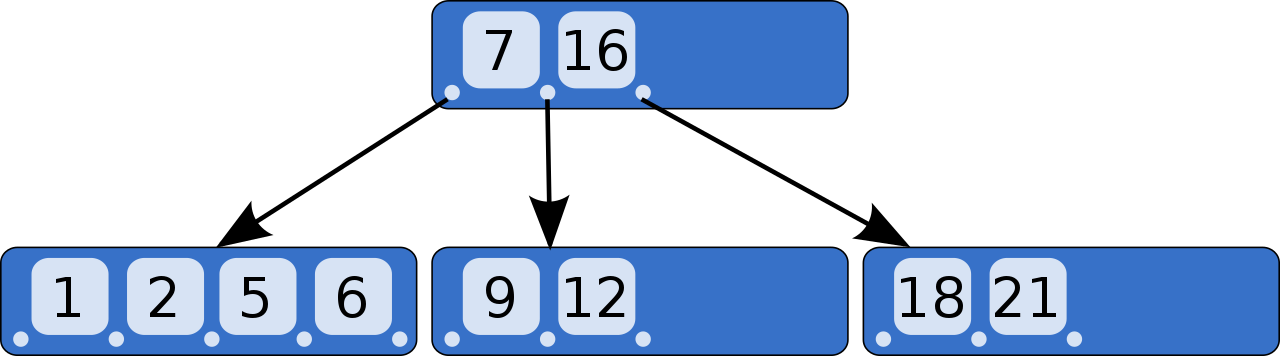
\includegraphics[scale=0.25]{2.png}
\end{center}
\paragraph{Analysis}
$n = (1 + \epsilon)M$ with $\epsilon > 0$ data outside of the memory. So $M$ is totally full and $\epsilon M$ is stored in the unbound memory.\\
The first point is we want to find $P($accessing the disk$)$, with a totally random algorithm, is $= \frac{\epsilon M}{n} = \frac{\epsilon\not M}{(1 + \epsilon)\not M} = P(\epsilon)$\\\\
The second point is the average time of a step. $\sum_x P(X = x)\cdot x$ with $X$ the variable of which we compute the average with that formula. $X$ is time, in this case. The time is $1$ in case of computing, and varies in case of accessing the memory. So we have the multiply the cost of access times the probability (of computing, going internal, going to the disk). Internal memory access costs 1, while on disk is larger and we say that the cost is $c$. So the average, with let's say $a$ probability of memory access, $= (1 - a)\cdot 1 + a(P(\epsilon)\cdot c + (1 - P(\epsilon))\cdot 1)$ but $0 < a < 1$ and $1 - P(\epsilon)$ are very small, so we can rewrite as $= a\cdot P(\epsilon)\cdot c = a \cdot \frac{\epsilon}{1 + \epsilon} \cdot c + O(1)$. If $a = 0$ then no memory access so the cost is constant. The larger is $a$ the more memory access, the more the term is important, which is exactly what we want to capture. Usually, $a = 0.3 = 30\%$ and $c = 10^6$ the gap between accessing the disk and accessing the internal memory.\\
So $\frac{\epsilon}{1 + \epsilon}\cdot 0.3 \cdot 10^6 = \frac{\epsilon}{1 + \epsilon} \cdot 300000$. If $P(\epsilon) = 0.001$ the avg time of a step is $0.001 \cdot 300000 = 300$, so the disk has a lot of impact even with only a thousandth of memory access being on disk: the avg cost is 300 and not 1.
\section{Sorting}
\paragraph{Permuting problem} Given an array $S[1, m]$ and a permutation $\pi$, the permutation problem asks to permute $S$ according to $\pi$, creating $[S[\pi[1]], S[\pi[2]],\ldots,S[\pi[m]]$. For example $S = [A, B, C, D], \pi = [3, 1, 2, 4]$ then $\pi$ tells that the $\pi[0] = 3$ item goes to the first position. So $S_\pi = [C, A, B, D]$
\begin{lstlisting}[style=myPython]
for i = 1 to n:
	S1[i] = S[pi[i]]
\end{lstlisting}
Which costs $\Theta(n)$\\
\begin{tabular}{c | c | c}
 & PERM & SORT \\
\hline
RAM & $n$ & $n\log n$\\
\hline
2-level memory & min\{$n$, $C_{sort}$\} & $C_{sort}$
\end{tabular}
\pagebreak

Solving the permuting in a scan + sort kind of way, otherwise we have to do a disk access per value.\\
\begin{list}{}{}
	\item scan S : $\langle$S[i], i$\rangle$ which is $\langle$item, position$\rangle$\\
	Which creates $\langle$A, 1$\rangle$ $\langle$B, 2$\rangle$ $\langle$C, 3$\rangle$ $\langle$D, 4$\rangle$\\
	This costs $O(\frac{n}{B})$
	\item scan $\pi$ : $\langle\pi$[i], i$\rangle$ which is $\langle$src, dst$\rangle$\\
	Which creates $\langle$3, 1$\rangle$ $\langle$1, 2$\rangle$ $\langle$2, 3$\rangle$ $\langle$4, 4$\rangle$\\
	This costs $O(\frac{n}{B})$
	\item sort by first component of the sequence $\langle\pi$[i], i$\rangle$\\
	Which creates $\langle$1, 2$\rangle$ $\langle$2, 3$\rangle$ $\langle$3, 1$\rangle$ $\langle$4, 4$\rangle$\\
	We take the item in source and move to destination
	\item parallel scan
	$\langle$A, 1$\rangle$ $\langle$B, 2$\rangle$ $\langle$C, 3$\rangle$ $\langle$D, 4$\rangle$\\
	$\langle$1, 2$\rangle$ $\langle$2, 3$\rangle$ $\langle$3, 1$\rangle$ $\langle$4, 4$\rangle$\\
	Which creates $\langle$A, 2$\rangle$ $\langle$B, 3$\rangle$ $\langle$C, 1$\rangle$ $\langle$D, 4$\rangle$\\
	\item sort by second component\\
	Which creates $\langle$C, 1$\rangle$ $\langle$A, 2$\rangle$ $\langle$B, 3$\rangle$ $\langle$D, 4$\rangle$\\
	\item scan\\
	Which creates [C, A, B, B]\\
	This costs $O(\frac{n}{B})$
\end{list}
The I/O cost is 4 scan + 2 sort $= O(\frac{n}{B}) + 2\cdot O(C_{sort})$ sorting cannot cost less than $\frac{n}{B}$ because we can't improve that, so $O(C_{sort})$\\\\
So we have proposed upper-bounds = algorithms for the sorting and the permuting problem. The permuting problem can be solved in $O(\frac{n}{B}) +$ sorting I/Os. Moving $n$ items takes $\Theta(n)$ I/Os.\\
Sorting $n$ items in a two level memory of size $M$ for internal memory and $B$ for the disk page size, costs $O(\frac{n}{B} \cdot \log_{\frac{M}{B}} \frac{n}{M})$ with $L = \log_{\frac{M}{B}} \frac{n}{M}$, and often written as $\overline{O}(\frac{n}{B})$ with the overline or over tilde that means that is a scan.\\
$L$ consists of the base $\frac{M}{B}$ and the argument $\frac{n}{B}$ which means that with a larger memory I'd like it to be faster, with bigger $M$ the argument decreases and the base increases so the logarithm shrinks a lot. With a bigger $B$ page size, $\frac{n}{B}$ decreases but the base increases.\\
$\frac{M}{B} =$ how many pages I can keep in the internal memory. Let's say $n = 2^{40}$, $M = 8$Gb $= 2^{33}$ and $B = 32$Kb $= 2^{15}$, then $$\log_{\frac{n}{B}} \frac{n}{M} = \frac{\log_2\frac{n}{M}}{\log_2 \frac{M}{B}} = \frac{\log_2 \frac{2^{40}}{2^{33}}}{\log_2 \frac{2^{33}}{2^{15}}} = \frac{\log_2 2^7}{\log_2 2^{18}} = \frac{7}{18} < 1$$
Let's see when is sorting preferred to moving items or viceversa
$$\frac{n}{B} \log_{\frac{M}{B}} \frac{n}{M} < n \Leftrightarrow \log_{\frac{M}{B}} \frac{n}{M} < B$$\\
We have $B = 1$ in the RAM model, $B = 32$Kb in the 2-level model compared to $\log_{\frac{M}{B}}\frac{n}{M} = 2$ or $3$. In practical situations with disk, sorting is better than moving numbers. If $B = 1$, in the RAM model, $M = O(1)$, then sorting is worse than moving.
\paragraph{Sorting} Let's consider binary merge sort, which in the worst case costs $O(n\cdot \log_2 n)$.
\begin{lstlisting}[style=myPython]
def MergeSort(S, i, j):
	if (i < j):  # sort if at least two items, otherwise already sorted
		m = (i+j)/2
		MergeSort(S, i, m-1)  # split into two halves
		MergeSort(S, m, j)
		Merge(S, i, m, j)  # most of the cost is here
\end{lstlisting}
Let's evaluate the I/Os in the case that $n >> M$ so the array can't be stored entirely in internal memory. Since it's based on the merge procedure, we can evaluate the cost of the merge and multiply by the number of levels. It loads a page every time it needs it and writes a pages every time it fills one. So if the two arrays to merge are long $l$, it makes $\frac{l}{B}$ I/Os. So it takes $O(\frac{n}{B} \log_2 n)$ I/Os.\\
Sorting = computing the sorted permutation + implement the sorted permutation. So we can say that sorting $\geq$ permuting, is at least difficult as permuting.\\
In the RAM model the $\geq$ is $>$, it's strict, because sorting is $n\cdot\log n$ and computing is the real issue, because implement is linear. In the 2-level memory model they are almost equivalent. This considering \textbf{atomic items}, integers o non-splittable strings.\\
The mismatch is the base of the logarithm. The binary merge sort is $O(\frac{n}{B} \log_2 \frac{n}{M})$: partitioning the array in blocks of size $M$, the size of the memory, called runs. Can we generate runs longer than M in few I/Os? On average we will be able to create runs of size $2M$, which saves 1 full scan of data (which, for large data, is a lot of time saved).
\paragraph{Snow plow algorithm} Sort item that you can, leave item that you cannot.\\
S = 1, 7, 5, 3, 2, with M = 3 items. The memory is divided in two parts: a min heap, items that are still unsorted, and an unsorted part, the snow that we cannot clean. Start from the memory with everything unsorted: min heap empty and only unsorted items. We put $M$ unsorted items, so 1, 7, 5 in the unsorted part. We sort the unsorted items and move to the min heap, with the unsorted part left empty. We pick the minimum element and write it out of the memory. We have emptied a position, and we can fetch another item in the unsorted part, the 3. The new item is compared to the minimum. 3 is larger than the current minimum, so is written inside the min heap, which is now 3, 5, 7. We write again out the minimum, 3, and fetch another item. 2 is smaller than 3, so it goes in the unsorted part. At some point the min heap will be empty, the unsorted part will be full and we restart the phase. We pay 1 I/O as soon as we write out $B$ items.
\begin{center}
	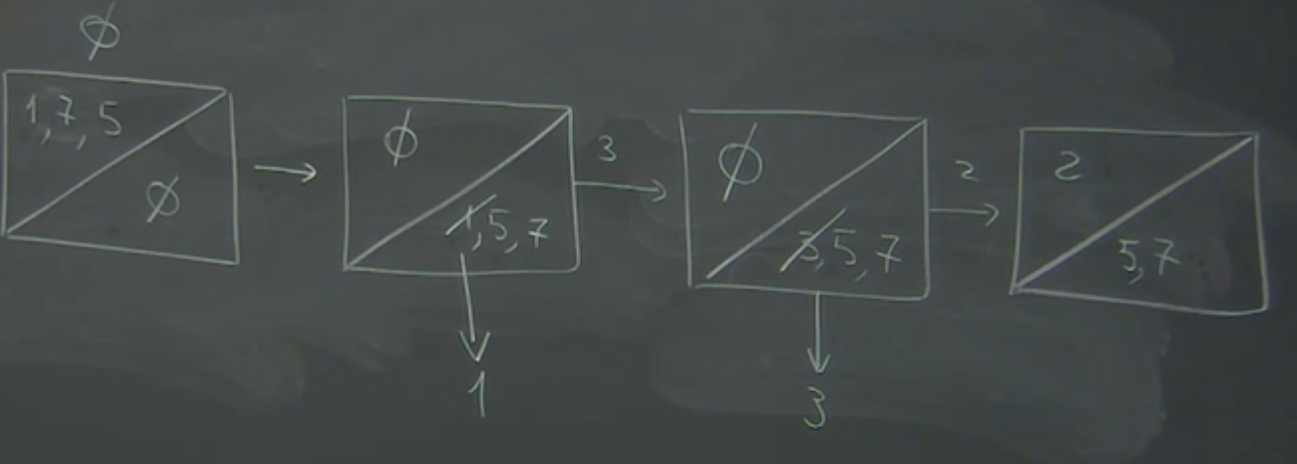
\includegraphics[scale=0.5]{1.png}
\end{center}
\begin{lstlisting}[style=myPython]
U = unsorted array of M items
H = min-heap over items of U
U = {}
while H != {}:
	min = minimum from H
	min -> output run
	next = next item from input sequence
	if next < min:
		next -> U
	else:
		next -> H
\end{lstlisting}
Let's prove that the runs are 2M on average. We start with $|U| = M$ and $|H| = 0$, with U unsorted part and H heap part. Continuing we read items, with $\tau = \#$ items read. The phase has processed $\tau + M$ items, $\tau$ read and $M$ already in memory. At the end of the phase, the min heap is empty $|H| = 0$ and $|U| = M$ and $\tau$ items are written out. So $\tau$ is the length of the run, we have to compute it, by making hypothesis about the distribution of the items, the probabilities of going to $U$ and $H$. $P($item read goes to $U) = \frac{1}{2}$, a totally random situation. By changing the probability we change "how much sorted" is the sequence. The more sorted is the sequence, the smaller the probability of going to $U$. avg$(|U|) = E[|U|] = \tau/2$ because we have $\tau$ items that go to $U$ with probability $\frac{1}{2}$.\\
Given that $|U| = M$, then on average $E[|U|] = \frac{\tau}{2} = M$ so average $\tau = 2M$
\paragraph{Exercise} $M = 2$ and $S = 1, 8, 3, 2, 5, 0, 4, 6$\ldots
\paragraph{Issues} Binary Mergesort doesn't always exploit all the memory. Because after creating the $M$-long first runs, by merging we need $3B$ for reading the memory (one for the first run, one on the second run and one page on the output), so $3B << M$, a lot of unused memory. We could fetch 2 pages per run, but the second page can be used only after the first page, so no advantage in allocating all data. Since there's a sequence of processing, even if a load immediately all the pages, we do not have much advantage in doing so. So we would like to merge $k$ runs instead of two runs at a time. Since we want to fill the memory, we want $(k+1)B = M$, $k$ pages for $k$ runs plus an output page. So $k = \frac{M}{B} - 1$ which we can approximate with $\frac{M}{B}$. Each run generates $\frac{1}{B}$ I/Os, and the merged run is long $k\cdot\frac{M}{B}$ elements.\\
So every run is of $M$ elements which take $\frac{M}{B}$ I/Os, for $\frac{n}{M}$ runs. So the total cost is $O(\frac{n}{\not M} \cdot \frac{\not M}{B}) = O(\frac{n}{B})$ for creating runs. So the merge tree has $\frac{n}{M}$ leaves and every node has $k$ runs to merge from the lower level, making it $\log_k \frac{n}{M}$ levels high.\\
The cost of mergesort is $O(\frac{n}{B} + \frac{n}{B}\cdot\log_k \frac{n}{M})$ which we have seen with $k = \frac{M}{B}$. It's the cost of creating the runs ($\frac{n}{B}$) plus the cost of merging (every merge is linear, total length divided by $B$, by the number of merge operations which is the levels of the tree)\\
With improve B, M by compression. So 3, 5, 10 is written as 3 (the first item) and storing the gaps (gap encoding) so 2, 5,\ldots with variable length encoders.\\\\
Let's rewrite the bound
$$\frac{n}{B}\cdot\log_{\frac{M}{B}}\frac{n}{M}$$
We don't know how items are consumed on the disks, given $D$ disks. With $k = 2, D = 2$ we can take advantage of the parallelism on the first load. But once loaded in memory, we may consume the pages asymmetrically, so we may end up reading a lot from a disk and very few times from the other. Possibly, every page on the first disk is used before the second page on the second disk. So by adding more disks we take full advantage because they are the denominators. The know optimal bound is:
$$\Theta\left(\frac{n}{BD}\cdot\log_{\frac{M}{B}}\frac{n}{BD}\right)$$
For 1 disk is $O(\frac{n}{B}\cdot\log_{\frac{M}{B}}\frac{n}{B})$\\
For $D$ disks we can consider one big disk with $B' = D\cdot B$ page size, so the heads of the disks are fixed together and move together. We do not change the algorithm, so the complexity is simply $O(\frac{n}{B'}\cdot\log_{\frac{M}{B'}}\frac{n}{B}) = O(\frac{n}{DB}\cdot\log_{\frac{M}{DB}}\frac{n}{DB})$ but with D in the base of the logarithm makes the value larger, but the impact is small and the simplicity of the method makes it worth it. This is called \textbf{disk striping}.
\paragraph{Binary Decision Trees} Every node $(a,b)$ generates a comparison, the left branch is followed if $a<b$ and the right if $a>b$: it represents an algorithm. The leaves are sorted permutations according to the path of comparisons, total number of leaves is $n!$. The question is how big should be the tree so that it's a sorting algorithm, so to reach a number of leaves that's at least $n!$? It grows by $2^t$ nodes for every level $t$, so $2^t > n!$ and we have the lower bound.\\
The left subtree, where the comparison is $a < b$, simply generates (by following a path) all the permutations in which $a$ comes before $b$, whatever number of elements are between them. The right path, vice versa, generates permutations where $b$ comes before $a$.
\paragraph{Lower bounds} There are also lower bounds about permuting, an extra for the oral.\\
Binary decision trees proved lower bound of sorting in the RAM model. Now let's see the I/O lower bound, so not counting comparisons but read/written pages. The main idea is that whenever I fetch a page I fetch $B$ items, not just two, so we can do many comparisons before loading another page. And the page goes in internal memory where there are more items which we compare. Whenever the items goes to internal memory we have to avoid repeating comparisons.\\
The memory $M$ consists of several items, we bring the page of size $B$ in internal memory and we have $M-B$ other items in the memory. One I/O executes many comparisons. If $B = 1$ and $M - B = 3$, so 3 items in $M$ and 1 item brought from disk. How many comparisons? We can assume that the items in memory are sorted, so the item brought can go in 4 position (before the first, between the first two\ldots). In general, the $B$ items can enter the $M-B$ items in $n$ ways. The memory consists of $M$ cells, so $n = \left(\begin{array}{c}
M\\B
\end{array}\right)\cdot B!$ with $B!$ because we have to account for the shuffling, so it needs to be counted only once. We have $\left(\begin{array}{c}
M\\B
\end{array}\right)$ because every item from $B$ can be inserted in one slot of $M$ possible slots, so $B$ slots out of $M$.\\

\pagebreak
So two situations \begin{enumerate}
	\item A new read, a read of an input page for the first time\\
	\# new reads = $\frac{n}{B}$
	\item An old read, all other read-cases, $t - \frac{n}{B}$
\end{enumerate}
$t$ I/Os, can be a new or an old read. Either one of the $\frac{n}{B}$ pages for the first time or any other page (or one of those pages for the second/third/\ldots time).\\
Two kinds of nodes, one node refers to a new I/O the other to an old I/O.\\
In a new I/O we have $\left(\begin{array}{c}
M\\B
\end{array}\right)\cdot B!$ options, we have to account for the shuffling, in the second case we have $\left(\begin{array}{c}
M\\B
\end{array}\right)$ options.\\
So in any path $\frac{n}{B}$ are new and $t - \frac{n}{B}$ are old. So how many steps or levels $t$ are needed to guarantee that the number of leaves is $\geq n!$? Every node is no longer binary and can be one of two kinds. Still a decision tree. So in every step we have $\frac{n}{B}$ new I/Os and $t - \frac{n}{B}$ old I/Os.\\
\# permutations that the algorithm can distinguish is $$= \left( \left(\begin{array}{c}
M\\B
\end{array}\right)\cdot B!\right)^{\frac{n}{B}}\cdot \left(\begin{array}{c}
M\\B
\end{array}\right)^{t - \frac{n}{B}} = \left(\begin{array}{c}
M\\B
\end{array}\right)^{t}\cdot \left(B!\right)^{\frac{n}{B}} \geq n!$$
To compute, consider that $\log\left(\begin{array}{c}
a\\b
\end{array}\right) = b\log_2 \frac{a}{b}$ and solving for $t$ gives the multi way merge sort bound. $t = \Omega(\frac{n}{B}\log_{\frac{M}{B}} \frac{n}{M})$
\paragraph{Two sorting paradigms} The following:
\begin{list}{}{}
	\item merge-based paradigm: partition (computationally free, $O(1)$), recursion, recombination (merge, $O(\frac{n}{B})$)
	\item distribution/partitioning-based paradigm: partition (costly part, $O(n)$), recursion, recombination ($\not\exists$)
\end{list}
How can we design a multi way quick sort? We can't take one pivot, because that'll be binary. We can take many pivot but we have to guarantee a good usage of internal memory, but more importantly we need that the partition have to balanced: with $k$ pivot I'd like that every partition has $\frac{n}{k}$ items. This requires a theorem.\\
Let's refresh the quick sort. %TODO
\paragraph{Time complexity of quick sort is $O(n\log n)$} Let's prove it by introducing a random variable\\ $X_{u,v} = \left\{\begin{array}{c l}
1&\hbox{if }S[u]\hbox{ is compared to }S[v]\\0&else
\end{array}\right.$ and we want the average number of comparisons $$E\left[\sum_{u=1}^m\sum_{v>u}^m X_{u,v}\right] = \sum_{u=1}^m\sum_{v>u}^m E\left[X_{u,v}\right] = $$
The average of an indicator value (which $X_{u,v}$ is) is the sum of all possible values times their probability $$= \sum_{u=1}^m\sum_{v>u}^m \left(1\cdot P(S[u]\hbox{ is compared to }S[v]) + 0\cdot P(S[u]\hbox{ is not compared to }S[v])\right) = $$
$$=\sum_u \sum_v P(S[u]\hbox{ is compared to }S[v])$$
Let's focus on the probability that taken two items they are compared. Comparison in quick sort is particular, may only occur in the partition part and when one of the elements is a pivot. With just one pivot and two parts, then $S[u]$ is compared to $S[v]$ only when one of them is the pivot. So $P(S[u]\hbox{ is compared to}S[v]) = P(S[u]$ or $S[v]$ is choosen as pivot in one call that involves both of them$)$
\begin{list}{}{}
	\item Case $a$: the pivot is smaller or greater than both items, so both items go to the same partition: not significative because they can be compared in the next time 
	\item Case $b$: the pivot is between the two items, so no comparison because they'll go to different partitions.
	\item Case $c$: is that one of the two items is taken as pivot, so \textbf{there's the comparison}.
\end{list}
So the probability is the number of times that $c$ can happen (two items, so $2$) divided by the total number of events possible, $b + c$, which is any item choosen between the two elements included, so $S[v] - S[u] + 1$. So $P(S[u]\hbox{ is compared to }S[v]) = P(S[u]$ or $S[v]$ is choosen as pivot in one call that involves both of them$) = \frac{2}{S[v] - S[u] + 1}$\\
\paragraph{$k$th ranked item} In unsorted array $S$: is the item that, taken $S$, would go to the $k$th place is $S$ would be sorted. The obvious way of finding out would be to sort and pick the item in the position $k$, but you'd be paying $n\cdot\log n$. This problem can be solved in linear time $O(n)$ on average: same base as quick sort with just one recursive call. Pick a random pivot and do a three-way partition: a partition of $n_<$ smaller elements than the pivot, a partition of $n_=$ elements of the same value as the pivot and a partition of $n_>$ larger elements than the pivot. Of course the left and right partition, of respectively smaller and bigger elements, are unsorted (the middle partition is of equal elements so is trivially sorted) but if the elements falls into the middle partition we can immediately know which elements it is. For example, $[3,2,0,\vline7,7,7,\vline10,8,9]$, if $k$ is 4 we can answer that, being that there are $3$ elements in the left partition, the 4th ranked element is a 7. Then if $k$ falls in the $=$ partition, I'm done. If it falls in one of the other two, I cannot know but we can already discard some items: if the pivot is in the $<$ part we recurse on that part, otherwise if the pivot is on the $>$ part we recurse over there (in this case, dropping from $k$ the items that are smaller, so $k = k - n_= - n_<$). Only one recursive call.\\
$T(n) = O(n) + [T(n_<)$ or $T(n_>)]$ choice of going to the left or to the right, probability. Let's analyze that probabilities. Supposing that $n_= = \frac{n}{3}$, a balanced partitioning, with the pivot falling among the $n_=$ items (the middle partition). So this is the good case: the pivot is between the position $\frac{n}{3}$ and $\frac{2}{3}n$, and happens with probability $\frac{1}{3}$. The bad case is the pivot falling into the left or right partition.\\
In the good case $n_< \leq \frac{2}{3}n$ and $n_> \leq 	\frac{2}{3}n$. So $$T(n) = O(n) + (P(\hbox{good case})\cdot T() + P(\hbox{bad case})\cdot T()) \Leftrightarrow$$
$$\Leftrightarrow T(n) = O(n) + \left(\frac{1}{3}\cdot T\left(\frac{2}{3}n\right) + \frac{2}{3}\cdot T(n - 1)\right) \Leftrightarrow$$
$$\Leftrightarrow T(n) \leq O(n) + \frac{1}{3}\cdot T\left(\frac{2}{3}n\right) + \frac{2}{3}\cdot T(n) \Leftrightarrow$$
$$\Leftrightarrow \frac{1}{3}T(n) \leq O(n) + \frac{1}{3}\cdot T\left(\frac{2}{3}n\right) \Leftrightarrow$$
$$\Leftrightarrow T(n) \leq O(n) + T\left(\frac{2}{3}n\right)$$
\paragraph{Dual Pivot (2012)} 3-way partitioning made with 2 pivot taken at random: it reduces the number of comparisons and it increases the number of swaps. This seems totally ineffective (swaps impacts on memory and comparison on CPU), but the problem here is mispredictions on the CPU, modern CPU do look-ahead in the computing and if it badly predicts the future ifs it has to break the stack and go back. So with fewer comparisons it's better, it reduces the mispredictions. 10\% circa speed-up factor.\\
The pivots maintain an invariant: the first partition, until index $l-1$, are items smaller than the first pivot ($p$), then there's a partition of items $p\leq \ldots \leq q$ with $q$ being the second pivot and this partition starts at $l$ and ends at $k-1$. Then there's a partition of items that are still to be processed from index $k$ to $g$, and at the end a partition of elements $> q$.
\begin{center}
	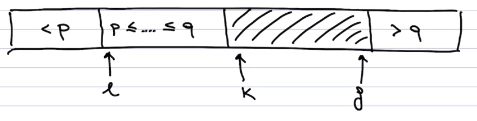
\includegraphics[scale=1]{7.png}
\end{center}
We take $S[k]$ and compare it to $p$. If $S[k]<p$ then swap (insert $S[k]$ in position $l$ and increase $l$). Else, we compare $S[k]$ with $q$. If $S[k]\leq q$ we don't have to do anything, it's already in the correct position. Else, $S[k] > q$: we start from $g$ and go back until we find an element $\leq q$ and we swap $S[k]$ with that element.
\paragraph{Bounded Quick Sort} Bounding the recursive calls. Transform the deepness of the tree (the number of recursive calls) from $n$ to $\log n$, but the time complexity remains $n^2$ in the worst case.\\
The trick is removing tail recursion. Techniques applied by compilers, we'll do by hand.\\
\begin{center}
	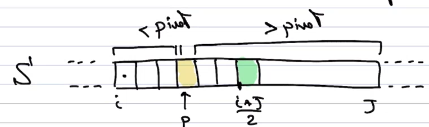
\includegraphics[scale=1]{8.png}
\end{center}
Generic call, between positions $i$ and $j$. If $j - i > n_0$ (so if is sufficiently small, the array is in cache so we go fast) then we do insertion sort.\\
In the other case, with $\frac{i+j}{2}$ being the middle element, we do the partitioning: assuming the pivot on the left of the middle ($i \leq p < \frac{i+j}{2}$), the left partition of the pivot is smaller so contains less than half elements. So $i \leq p < \frac{i+j}{2}$, then recurse on the left because it has fewer elements, but we do not recurse on the right because it has a lot of elements so after the recursive call on the left we simply move $i$ by doing $i = p + 1$. Else, with $p$ on the right part, recurse on the right partition and then do $j = p-1$
\paragraph{Multi Way Quicksort} Key idea, given that we have a long array $S$ to be sorted so doesn't fit in internal memory: we want to partition $S$ among $k$ buckets $B_1,B_2,B_3,\ldots,B_k$. Every bucket is associated to a pivot: $k-1$ pivots, a logical pivot $s_0 = -\infty$ at the beginning, $s_{k+1} = \infty$ at the end and $s_1,s_2,s_3,\ldots,s_{k-1}$ between the buckets.\\
$B_i=\{S[j]\:|\: s_{i-1} < S[j] \leq s_i\}$, so the "right" pivot is part of the bucket ($s_i \in B_i$). The goal is having balanced $B_i \forall\:i$, so $|B_i| = \frac{n}{k}$.\\
The idea is similar to marge sort but in reverse: we assume that in memory $M$ we have $k$ buckets of size $B$, so we want to guarantee that $k\cdot B \leq M$. We sample at random $(k-1)$ pivots from $S$ (done with a scan $O(\frac{n}{B})$ I/Os). Not easy, sampling at random, we will see. We sort the the pivots $s_1 < s_2 < \ldots < s_{k-1}$, with 0 I/Os because those are all in internal memory. But we cannot assume that the buckets in memory can contain the $S$'s buckets. So we fetch $B$ items from $S$ and distribute the items according to the pivots and do until a bucket is full. When a page is full, we write it as the first page of the corresponding buckets (according to the pivot). This takes $O(\frac{n}{B})$ I/Os.
\begin{enumerate}
	\item Pick at random $(a + 1)k - 1$ samples from $S$, the pivots $\Rightarrow A$
	\item Sort the samples in $A$
	\item $s_i = A[(a+1)i]$\\
	Until the last block has $a$ items
	\begin{center}
		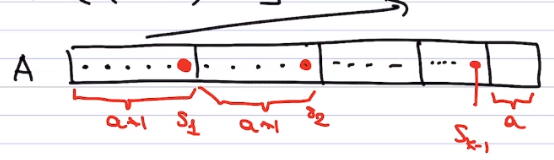
\includegraphics[scale=0.5]{3.png}
	\end{center}
	We sampled $(a+1)(k-1) + a = (a+1)k -1$ items
\end{enumerate}
If $a = 0$ the number of samples is $k-1$, no oversampling, fast sort ($O(k\log k)$) but no room to play around with the items. If $a > 0$ the sorting costs $O((ak)\log (ak))$. We chose $a = \Theta(\log k)$, only a logarithmic oversampling to get the balance $$a + 1 = 12\ln k$$ Balanced $\Rightarrow |B_i| < 4\cdot\frac{n}{k}$
\paragraph{Proof} By contradiction. We want to estimate $P(\exists\:B_i\:|\:|B_i|\geq \frac{4n}{k})$ and prove that it is $\leq \frac{1}{2}$ so that on average two extractions are enough to guarantee that one is correct.\\
$B_i = \{S[j]\:|\: s_{i-1} < S[j] \leq S_i\}$ by definition. $A_{sort}$  contains samples from $S$.\\
$S_{sort}$ is composed of $\frac{k}{2}$ cells of size $\frac{2n}{k}$: $t_0, t_1, \ldots, t_\frac{k}{2}$.\\
Some pieces of $t_i$ will be totally covered by a bucket $B_j$, because since $B_i$ has size of at least $\frac{4n}{k}$ it's not possible for it to be totally included into a $t_i$. $B_j$ has twice the size, so at least one $t_i$ will be totally covered by it. So this means that $P(\exists\:B_i\:|\:|B_i|\geq \frac{4n}{k}) \leq P(\exists\: t_j\:|\: t_j$ is covered entirely by some $B_i)$. So the element before the beginning of $B_i$, which is $s_{i-1}$, it's contained in some point of some $t_{j-1}$ and the last element, $s_i$, is in some part of $t_{j+1}$.
\begin{center}
	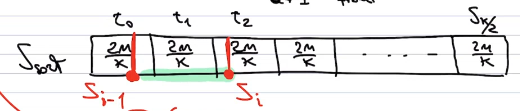
\includegraphics[scale=0.75]{4.png}
\end{center}
This means that the $a$ samples are distributed in that part, between $s_{i-1}$ and $s_i$: part in $t_{j-1}$, part in $t_j$ and part in the beginning of $t_{j+1}$. How many samples inside $t_j$, the block covered by $B_i$? They are surely $< a+1$, so\\$P(\exists\: t_j\:|\: t_j$ is covered entirely by some $B_i) \leq P(\exists\:t_j\:|\:t_j$ contains less than $a+1$ samples$)$\\
We now apply the \textbf{union bound}: the probability of existence is upper bounded by the number of possibilities times the probability of one of the events. So $P(\exists\:t_j\:|\:t_j$ contains less than $a+1$ samples$) \leq \frac{k}{2}\cdot P(t_1$ contains less than $a+1$ samples$)$. We need to estimate the latter, how many samples will go to $t_1$. $P($sample occurs in $t_1) = \frac{\frac{2n}{k}}{n} = \frac{2}{k}$, and the average number of samples in $t_1$, given $X_i = 1$ if the $i$th item is in $t_1$, is $X =$ \# of samples in $t_1 = \sum_{i = 1}^{(a+1)k - 1} X_i$. So $E[X] = E[\sum_i X_i] = \sum_{i = 1}^{(a+1)k - 1} E[X_1] = ((a+1)k - 1)\frac{2}{k} \geq 2(a+1) - 1$ because $k \geq 2$ and $2(a+1) - 1 \geq \frac{3}{2}(a+1)$.
\paragraph{} %TODO first part of 22/9 lecture
$P(p\in D) = $ positive events / total number $= \frac{|D|}{n} < \frac{m}{n} \leq \frac{\frac{n}{2}}{n} = 1$\\
%TODO algorithm and proof of 22/9

$n$ is known, streaming model, $M = 2$, $n = 8$ items which are $[a, b, c, d, e, f, g, h]$, $P = [.5, .5, 0, .5, 1, 0, 1, 1] \leftarrow Rand(0,1)$\\
$P($sample $i_j) = \frac{m - s}{n - k + 1}$ with $s$ being\\ %TODO
\begin{list}{}{}
	\item $s = 0, j = 1$ extracts a probability ($.5$) and compare $P$ against the $P($sample $i_j)$\\
	$P = .5 \leq \frac{2 - 0}{8 - 1 + 1} = \frac{1}{4}$, first item not picked
	\item $s = 0, j = 2, P = .5 \leq \frac{2 - 0}{8 - 2 + 1} = \frac{2}{7}$, not picked
	\item $s = 0, j = 3, P = 0 \leq \frac{2 - 0}{8 - 3 + 1} = \frac{1}{3}$, $c$ is picked
	\item $s = 1, j = 4, P = .5 \leq \frac{2 - 1}{8 - 4 + 1} = \frac{1}{5}$, not picked
	\item $s = 1, j = 5, P = 1 \leq \frac{2 - 1}{8 - 5 + 1} = \frac{1}{4}$, not picked
	\item $s = 1, j = 6, P = 0 \leq \frac{2 - 1}{8 - 6 + 1} = \frac{1}{3}$, $f$ is picked
	\item $M = 2$ and we've picked two items, the end
\end{list}
In the reservoir sampling, still streaming model but $n$ is unknown. $S = [a, b, c, d, e, f, g, h, i\ldots]$, $M = 3$. Reservoir initialized with first $M$ items, $R = [a, b, c]$. Each value in $S$ has an integer $\_, \_, \_, 2, 4, 1, 2, 3, 1$, with the last $1$ is the $h$ position, always drawn from the interval $[1, j]$. The number assigned are always smaller than the position $j$.
\begin{list}{}{}
	\item We consider the item $d$, extracts position $2 < 3 = M$ and substitutes $b$ in the reservoir, $R = [a, d, c]$
	\item $e$, position $4 > 3$ nothing changes
	\item $f$, position $1 < 3$ and substitutes $a$, $R =  [f, d, c]$
	\item $g$, $R = [f, g, c]$
	\item $h$, $R = [f, g, h]$
	\item $i$, $R = [i, g, h]$
\end{list}
\paragraph{Disk Striping} $D > 1$. Several disks, the pages of the disks are linked: first page of all $D$ disks are a single page. So it's considered as a single disk with $B' = D\cdot B$\\
In sorting, the bound is $O(\frac{n}{DB}\cdot\log_{\frac{M}{DB}} \frac{n}{M})$ over $D$ disks with disk striping. The lower bound is $\Omega(\frac{n}{DB}\cdot\log_{\frac{M}{B}} \frac{n}{M})$
$$\frac{\frac{n}{DB}\cdot\log_{\frac{M}{DB}} \frac{n}{M}}{\frac{n}{DB}\cdot\log_{\frac{M}{B}} \frac{n}{M}} \geq 1$$
$$\frac{\log_2 \frac{n}{M}}{\log_2 \frac{M}{DB}}\cdot \frac{\log_2 \frac{M}{B}}{\log_2 \frac{n}{M}}$$
$$\frac{\log_2 \frac{M}{B}}{\log_2 \frac{M}{B} - \log_2 D}$$
$$\frac{1}{1 - \frac{\log_2 D}{\log_2 \frac{M}{B}}}$$
$$\frac{1}{1 - \log_{\frac{M}{B}} D}$$
$\frac{M}{B}$ tipically thousands, $D$ at most 10-20, so $\log_{\frac{M}{B}} D < 1$. $M\to\infty \Rightarrow 1$ optimal. $M\to DB \Rightarrow \infty$, very very slow.
\section{Randomized data structures}
\subsection{Treap} From binary search TREe and hEAP.\\
Every node is divided in two part: one part is the key and the other is the priority. A treap is a binary search tree according to the key and a heap according to the priority. To distinguish, letters for the key and numbers for the priority and we consider a maximum heap.\\
Taken a node, in the left subtree the keys will be smaller than the root, the right will have larger keys. The left and right tree, being a maximum heap, have smaller priorities: so the root has the maximum priority.\\
Let's consider the following Treap:
\begin{center}
\Tree [.M,9 [.H,8 [.G,3 ] [.I,6 ] ] [.T,7 [.R,5 [.O,4 ] ] ] ]
\end{center}
The keys are given, but the priorities are extracted at random. So the idea is that whenever you have a key to insert, you draw at random a number that you associate to the key as a priority. The randomized priorities makes the Treap balanced on average.
\paragraph{3-Sided Range Query} We build a graph with the keys on the $x$ axis and the priorities on the $y$ axis.
\begin{center}
	\begin{tikzpicture}
		\begin{axis}[axis lines=middle,axis equal,grid=none,xticklabels={G,H,I,L,M,N,O,P,Q,R,S,T},xtick={1,2,3,4,5,6,7,8,9,10,11,12}]
		\addplot[mark=*] coordinates{(5,9)};
		\addplot[mark=*] coordinates{(2,8)};
		\addplot[mark=*] coordinates{(1,3)};
		\addplot[mark=*] coordinates{(3,6)};
		\addplot[mark=*] coordinates{(12,7)};
		\addplot[mark=*] coordinates{(10,5)};
		\addplot[mark=*] coordinates{(7,4)};
		\end{axis}
	\end{tikzpicture}
\end{center}
A typical query is indicated by $[a,b] \times [c,\infty]$, with $[a,b]$ on the $x$ axis and $[c,\infty]$ on the $y$ axis. The $x$ axis so is bounded, for example by $[L, P]$, and for example $[5, \infty]$ makes the priority of the query we are looking for start from $5$ upward. So the example becomes:
\begin{center}
	\begin{tikzpicture}
		\begin{axis}[axis lines=middle,axis equal,grid=none,xticklabels={G,H,I,L,M,N,O,P,Q,R,S,T},xtick={1,2,3,4,5,6,7,8,9,10,11,12}]
		\addplot[red, mark=*] coordinates{(5,9)};
		\addplot[mark=*] coordinates{(2,8)};
		\addplot[mark=*] coordinates{(1,3)};
		\addplot[mark=*] coordinates{(3,6)};
		\addplot[mark=*] coordinates{(12,7)};
		\addplot[mark=*] coordinates{(10,5)};
		\addplot[mark=*] coordinates{(7,4)};
		\addplot +[blue, mark=none] coordinates {(4, 0) (4, 11)};
		\addplot +[blue, mark=none] coordinates {(8, 0) (8, 11)};
		\addplot +[blue, mark=none] coordinates {(0, 5) (13, 5)};
		\end{axis}
	\end{tikzpicture}
\end{center}
The data structure should return the $M,9$ point, marked in the plot, because it's the only point in the set the resides in the query.\\
The root has highest priority, so in the plane is the top point. The left subtree is the subplot on the lower-left side of the root point, and the right subtree is the lower-right subplot
\begin{center}
	\begin{tikzpicture}
		\begin{axis}[axis lines=middle,axis equal,grid=none,xticklabels={G,H,I,L,M,N,O,P,Q,R,S,T},xtick={1,2,3,4,5,6,7,8,9,10,11,12}]
		\addplot[mark=*] coordinates{(5,9)};
		\addplot[mark=*] coordinates{(2,8)};
		\addplot[mark=*] coordinates{(1,3)};
		\addplot[mark=*] coordinates{(3,6)};
		\addplot[mark=*] coordinates{(12,7)};
		\addplot[mark=*] coordinates{(10,5)};
		\addplot[mark=*] coordinates{(7,4)};
		\addplot +[black, mark=none] coordinates {(4, 0) (4, 11)};
		\addplot +[black, mark=none] coordinates {(8, 0) (8, 11)};
		\addplot +[black, mark=none] coordinates {(0, 5) (13, 5)};
		\addplot +[blue, mark=none] coordinates {(5, 0) (5, 11)};
		\addplot +[blue, mark=none] coordinates {(0, 9) (13, 9)};
		\end{axis}
	\end{tikzpicture}
\end{center}
Then you recurse: find the root in the left subtree (topmost point) and create two other subplots \textbf{but limited to this subplot}. Example in the left subplot:
\begin{center}
	\begin{tikzpicture}
		\begin{axis}[axis lines=middle,axis equal,grid=none,xticklabels={G,H,I,L,M,N,O,P,Q,R,S,T},xtick={1,2,3,4,5,6,7,8,9,10,11,12}]
		\addplot[mark=*] coordinates{(5,9)};
		\addplot[mark=*] coordinates{(2,8)};
		\addplot[mark=*] coordinates{(1,3)};
		\addplot[mark=*] coordinates{(3,6)};
		\addplot[mark=*] coordinates{(12,7)};
		\addplot[mark=*] coordinates{(10,5)};
		\addplot[mark=*] coordinates{(7,4)};
		\addplot +[black, mark=none] coordinates {(4, 0) (4, 11)};
		\addplot +[black, mark=none] coordinates {(8, 0) (8, 11)};
		\addplot +[black, mark=none] coordinates {(0, 5) (13, 5)};
		\addplot +[black, mark=none] coordinates {(5, 0) (5, 11)};
		\addplot +[black, mark=none] coordinates {(0, 9) (13, 9)};
		\addplot +[blue, mark=none] coordinates {(2, 0) (2, 9)};
		\addplot +[blue, mark=none] coordinates {(0, 8) (5, 8)};
		\end{axis}
	\end{tikzpicture}
\end{center}
This was the approach in computational geometry, but the data structures are exactly the same.\\
So we start from the root, and we check if it's in the 3-sided range query. In this case is in the query, so we return it as a result. Since the root is inside the query, we go both left and right: this corresponds to going to the left and right subtree in the treap. In the left subtree, we recurs: is the root in the query? In this case, no but the height (priority) is still larger than the "bottom", the $c$ value, we go down. But we don't go to the left subtree (it's totally discarded) we go to the right subtree. If we went to the right subtree from the topmost root, that point it's still not in the query and still above $c$. Being in the right subtree, this time we go its left subtree and discard its right subtree. Basically we move toward the $b$ value when we are on the right and toward $a$ when we are on the left.\\
When we arrive in a node below the $c$ value we know that, being a maximum heap, everything below that has a lower priority so we can drop everything.\\
As for the \textbf{complexity}, we want to evaluate how much "wasted work" is done, as in how many nodes outside the query we evaluate. The number of points is equal to the depth of the tree, because we go only left or only right and always down one level, so given $h$ height of the treap, the number of extra points we check is $O(h)$, one node extra per level at most. Inside the query we evaluate both left and right subtrees, but those are all "good" points that go into the result, so it's no wasted work. The particular case happens when we check the node just above $c$ and in the query zone: for each of those nodes we check both subtrees, all of them will have priority $< c$ and will be cut out, but we check them. Those subtrees are at most twice the number of points of the result, the number of occurrencies. So the total number of work wasted is $h$ to the left $+ h$ to the right $2\cdot$occurrencies. The total cost then is $O(h +$ the number of occurrencies$)$. Of course the occurrencies cannot be avoided, as we have to list them.\\
The extra cost, $h$, is typically $\log n$ if the treap is balanced with $n$ being the number of points.
\paragraph{Rotation} Considering 
\begin{center}
\Tree [.$y$ [.$x$ [.\triangled{$\alpha$} ] [.\triangled{$\beta$} ] ] [.\triangled{$\gamma$} ] ]
\end{center}
In the right rotation, node $x$ goes up and node $y$ goes down. $\alpha$ was the left subtree of $x$ and remains that, same for $\gamma$ that remains the right subtree of node $y$. $\beta$ cannot remain linked to $x$ , so $\beta$ will be relocated as the left subtree of $y$.
\begin{center}
\Tree [.$x$ [.\triangled{$\alpha$} ] [.$y$ [.\triangled{$\beta$} ] [.\triangled{$\gamma$} ] ] ]
\end{center}
We claim that this relocation still guarantees the balancing of the treap. We can pick a node $k$ inside $\beta$
$$\hbox{key}(x) \leq \hbox{key}(k) \leq \hbox{key}(y)$$
because it's in the right subtree of $x$ (therefore, larger key) but it's inside the left subtree of $y$ (therefore, smaller key). When we go to $\beta$ as left subtree of $y$ after the rotation, so $y$ inside the right subtree of $x$, we have that a node $k$ inside $\beta$ satisfies the same condition: it's still in the left subtree of $y$, therefore has smaller key, and still in the right subtree of $x$, therefore greater key. So the relocation preserves the conditions.\\
It's constant time, $O(1)$, because we change a constant number of pointers.
\paragraph{Search($k$)} It's just the search in the binary search tree. Based on the searched key, we go on the left if it's smaller and on the right if it's larger, so priority is not needed. Cost is $O(h)$ with $h$ being the height of the tree.
\paragraph{Insertion($k, p$)} For example inserting $(S,6)$. We start by searching for the position of $S$ in the tree. Bigger than M, smaller than T, larger than R and empty so that's the spot.
\begin{center}
\Tree [.M,9 [.H,8 [.G,3 ] [.I,6 ] ] [.T,7 [.R,5 [.O,4 ] [.S,6 ] ] ] ]
\end{center}
It's still a binary search tree but it's not an heap because the priority 6 doesn't satisfy the condition. So like in the heap we have to check the balance: S,6 needs to go up but we have to preserve the heap property so we apply a rotation, in this case a left rotation because it's the right child.
\begin{center}
\Tree [.M,9 [.H,8 [.G,3 ] [.I,6 ] ] [.T,7 [.S,6 [.R,5 [.O,4 ] ] ] ] ]
\end{center}
So it's a search plus rotation to reestablish the heap property. The rotation is constant, but in the worst case there are $h$ rotations. So the cost is again $O(h)$.
\paragraph{Delete($k$)} The deletion is trivial when we delete leaves. But for example let's remove T: we can make it a leaf by setting the priority to $-\infty$. So deletion is just: search for $k$, set the priority to $-\infty$ and then apply rotations to reestablish the heap property, then delete. Again, $O(h)$.\\
Of course in this particular case T has just one child, so we could remove it and link S as right subtree of M, but the procedure above handles every possible case.
\paragraph{Merge$(T_1,T_2)$} $\forall\:x\in T_1$ and $\forall\:y\in T_2$ we have $\hbox{key}(x)<\hbox{key}(y)$.\\
We create a root with a logical key between the maximum key of $T_1$ and the minimum key of $T_2$ and $-\infty$ as the priority. The problem is the priority: it's a binary search tree (both $T_i$ are, and the chosen key mantains that condition) but the $-\infty$ priority breaks the heap condition. But we know we can apply rotations to reestablish the condition: the root goes down until it reaches the leaf level, where it can be dropped. When this happens, the rest of the "stuff" will be a treap. So again it's $O(h)$: creating the node it's constant and the rotations are $O(h)$.\\
The reverse operation is the split.
\paragraph{Split($k, T$)} Splitting $T$ according to the key $k$ means creating a treap $T_{<k}$ with keys $< k$ and another treap $T_{>k}$ with keys $> k$. This assuming $k\not\in T$. The split is trivial when the key is the root, so I need to put myself in a situation where $k$ occupies the root. So we first insert $k,\infty$, so that it goes to the root. At insertion, $k,\infty$ will be a leaf, so we rotate to reestablish the heap priority, arriving in a situation where we have $k,\infty$ as root with a left and a right subtree. The left subtree will be $T_{<k}$ and the right subtree will be $T_{>k}$ so the we delete the root. This costs $O(h)$ for insertion, $O(h)$ for rotations and constant for deleting the root, overall $O(h)$.
\paragraph{On average, a treap is balanced} By drawing the priorities at random, the average treap is balanced. $h$ height of the treap, it's $n$ if it's just a path or $\log n$ if it's balanced, but $h = O(\log n)$ on average. Let's prove it.\\
Let's create an indicator variable $A_k^i = \left\{ \begin{array}{c l}
1&\hbox{if }x_i\hbox{ is a proper ancestor of }x_k\\
0&\hbox{otherwise}
\end{array}\right.$\\
$depth(x_k) = \sum_{i=1}^k A_k^i$ which counts the proper ancestors of $x_k$. $E[depth(x_k)] = E(\sum_{i=1}^k A_k^i] = \sum_{i=1}^k E[A_k^i]$ and the expected of a indicator variable is the probability of it being 1 so $= \sum_{i=1}^k P(A_k^i = 1)$ which is the probability of $x_i$ being on the path to $x_k$. We consider $X(i,k)=\{x_i,x_{i+1},\ldots,x_{k-1}, x_k\}$ sorted. So $\sum_{i=1}^k P(A_k^i = 1)$ we consider $x_i < x_k$ or vice versa, is totally symmetric. So $priority(x_i) > priority(x_k)$\\
Theorem: $\forall\: i \neq k$ we have that $x_i$ is a proper ancestor of $x_k \Leftrightarrow priority(x_i)$ is the largest in $X(i,k) = \{x_i,\ldots,x_k\}$. In the minimum heap the priority would be the smallest.\\
Various cases:
\begin{enumerate}
	\item $x_r$ with largest priority, so $x_r,\ldots, x_i,\ldots, x_k$, so $x_r$ becomes the root of the treap and the $x_i,\ldots, x_k$ go to the right subtree. So we consider the subtree.\\
	Same for $x_r$ with largest priority and $x_i,\ldots, x_k,\ldots, x_r$. $x_r$ still root and $x_i,\ldots,x_k$ in the left subtree.\\
	So we restrict the attention to the $X(i,k)$ set.
	\item $x_i$ has the largest priority $\Rightarrow x_i$ is the root of the treap and $x_k$ goes to the right, so $x_i$ is the ancestor.
	\item $x_j$ has the largest priority, where $x_j\neq x_i$ and $x_j \in X(i,k)$, it's one of the items $\Rightarrow x_j$ to the root, $x_i$ to the left and $x_k$ to the right. So $x_i$ is surely \textbf{not an ancestor} of $x_k$.
\end{enumerate}
$P(x_i$ ancestor of $x_k) = P(x_i$ has the largest priority of $X(i,k))$ and because the priorities are picked are random $= \frac{1}{|X(i,k)|} = \frac{1}{k - i + 1}$ if $i < k$ or $\frac{1}{i - k + 1}$ if $i > k$. Not $\frac{1}{n}$ because we consider only the subset of $X(i,k)$\\
$\sum_{i=1, i\neq k}^n \frac{1}{|X(i,k)|} = \sum_{i = 1}^{k-1} \frac{1}{k-i + 1} + \sum_{i = k+1}^n \frac{1}{i - k + 1}$ the first goes like $\log_2 k$ (because it goes like $\frac{1}{k} + \frac{1}{k-1} + \ldots + \frac{1}{2}$) and the second goes like $\log_2 (n - k + 1)$ (because it goes like $\frac{1}{2} + \frac{1}{3} + \ldots + \frac{1}{n-k+1}$)\\
Keys are inserted in random order so that priority = order, so average depth is $O(\log n)$.
\subsection{Skip lists} We have a list of items $L_0 = -\infty \rightarrow 3 \rightarrow 6 \rightarrow 7 \rightarrow 10 \rightarrow 15 \rightarrow 16 \rightarrow +\infty$ with $\pm\infty$ logical marks. The search in lists is very bad, the idea is to create levels of lists. List of level $L_1 = -\infty \ldots +\infty$ with vertical pointers.
\begin{center}
	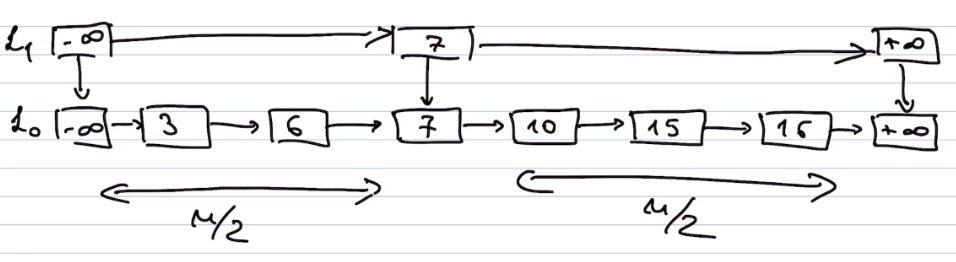
\includegraphics[scale=0.5]{5.png}
\end{center}
We can promote $k$ items to $L_1$, $k + \frac{n}{k} \Rightarrow k = \sqrt{n}$. The item are promoted randomly. For every item in $L_0$, it is promoted with probability = $\frac{1}{2}$ (coin toss, tails promotes heads doesn't), promoting $\frac{n}{2}$ items on average. This can be done for more levels.
\begin{center}
	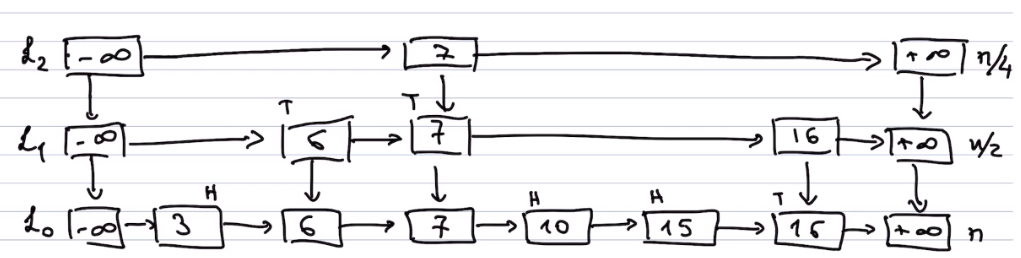
\includegraphics[scale=0.5]{6.png}
\end{center}
\paragraph{Search} We search for the topmost list, compare and go to the correct portion in the list below. At every step I scan the list if the element I'm looking for is larger and go to the list below if it's smaller.
\paragraph{Deletion} The deletion removes the column of items, in every list that item appears. In the worst case we reconstruct $\log n$ lists.
\paragraph{Insertion} First you find the position in $L_0$ (search, beginning from the topmost list), you insert and then toss the coin to insert in the upper list. To identify the left/right part in the upper list, we look for the latest item for every level that I have seen before going down during the search phase, in a sense that's the frontier to the item to be inserted.
\begin{center}
	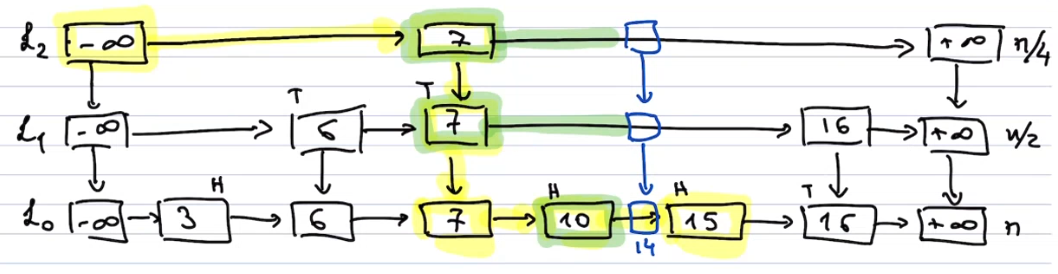
\includegraphics[scale=0.5]{9.png}
\end{center}
So keep track of the items that go down and adjust the pointers of those items.
\paragraph{Height of the skip list} $L =$ \# of levels of the skip list on $n$ items $= max_k L(k)$ with $L(k) =$ level of the $k$th item. So the height of the skip list, the levels of the skip list, is the maximum level among the items.\\
$P(L(k) \geq l) = $ the probability of extracting $l$ tails (independent coin tosses) $= \left(\frac{1}{2}\right)^l$.\\
$P(L \geq l) = P(max_k L(k) \geq l) = P(\exists\: k\:|\: L(k) \geq l) \leq n\cdot\left(\frac{1}{2}\right)^l = \frac{n}{2^l}$ for the union bound.
\begin{enumerate}
	\item $l \leq \log_2 n \rightarrow \frac{n}{2^l} \geq \frac{n}{2^{\log n}} = \frac{n}{n} = 1$ so the inequality is not significant, because a probability is always $\leq 1$
	\item $l > \log_2 n \rightarrow \frac{n}{2^l} < \frac{n}{2^{\log n}} = 1$
\end{enumerate}
$P(L \geq c\cdot\log_2 n) \leq \frac{n}{2^{c\cdot\log_2 n}} = \frac{n}{(2^{\log n})^c} = \frac{n}{n^c} = \frac{1}{n^{c-1}}$\\\\
In the search process we have, with high probability, $O(\log n)$ "down steps". For the number of "right steps", let's observe the process in reverse: from the bottom we go to the left for as many right pointers we find, but we god up as soon as we find a downward pointer. How many right pointers before a vertical pointer on average? We go left when we don't have a vertical pointer, which means with probability $\frac{1}{2}$ because of the coin toss, so it's a sequence of heads terminate by a tail (which means going up) so on average we have $2$ right steps. Every level is independent, so it applies to every level.\\
So $O(\log n)$ down steps and $O(\log n)$ right steps for the search process, so the total cost of search is $O(\log n)$. Insertion is a search plus a constant number of pointers change, deletion is a search plus a constant number of pointers change so everything is $\log n$.
\section{Set Intersection}
From a mathematical point of view we have $A,B\subseteq N$ and we want to compute $A \cap B$ fast. With $|A| = n, |B| = m$, in the case of unsorted sets, the comparison has complexity of $O(n\cdot m)$. We assume sorted sets, so we first sort $A$ and $B$ and then apply one of the algorithms that we'll see.
\subsection{Merge Based Intersection}
Based on the merge procedure seen in merge sort. For example $A = \underline{1},5,8,9,\ldots$ and $B = \underline{2}, 5, 9,\ldots$ with pointers on $1\in A$ and $2\in B$, the first elements. In the merge sort we do the comparison and write the minimum, advance the pointer in the corresponding list and go on. In the example we would end up with $1, 2, 5, 5, 8,\ldots$ But we want to simplify this. In this algorithm, whenever two items are compared, the minimum one is discarded and if the items are equal then it goes into the intersection.\\
It's linear in both lists, so the complexity is $O(n + m)$. This approach is optimal whenever $n$ is in the same order of $m$, or equal.
\subsection{Binary Search} Assuming $n > m$. We take an element from $B$ and binary search in $A$, for each element of $B$. Every search takes $\log n$, so this costs $O(m\cdot\log n)$. This approach is better than the previous, of $O(n + m)$ complexity, when $m\log n < n \Leftrightarrow m < \frac{n}{\log n}$. So it's better up to a very long $B$, which means that doing a continuous binary search is better than the merge based intersection.\\
This is true in theory, in practice scanning (the merge based intersection) is typically very fast.
\subsection{Mutual Partitioning} Still $n > m$. Let's say we take the first item of $B$, binary search over $A$ and find that it's between two certain values in $A$. When we pick the second item of $B$, in the binary search we start from scratch, but it's nonsensical because the second item is larger than the previous item of $B$, so we can search only in the last right partition of $A$ that's left. This way we always go to the right, but if the first item is at the beginning of $A$ we don't advance very much so we try to balance the partitioning: instead of picking the first element of $B$, we pick the middle element in position $\frac{m}{2}$. That middle element is found to occur between two elements in $A$, and this splits $A$ into $A_1$, until the left element included, and $A_2$ from the right element included. This also splits $B$ into two parts: the left half until the middle element excluded, $B_1$, and the right half from the middle element excluded, $B_2$.\\
After $\log n$ steps, the binary search, we have turned $A \cap B$ into two problems: $A_1 \cap B_1$ and $A_2 \cap B_2$, over which we can recurse.\\
We have that $|B_1| = |B_2| = \frac{m}{2}$, with a $\pm 1$ in case of odd $m$. Those two partitions will be again divided, and so on. So we make $\log m$ recursive steps. So the complexity $T(n, m) = O(\log n)$ (for the binary search) $+ T(n_1, \frac{m}{2})$ (for recursion over $A_1 \cap B_1$) $+ T(n_1, \frac{m}{2})$ (for recursion over $A_2\cap B_2$). To solve this we have to make some assumptions:
\begin{list}{}{}
	\item If the partitioning is fully unbalanced (the middle element of $B$ goes either all the way to the left or all the way to the right of $A$)\\
	 It's a good case because, although we keep all $A$ we still drop half of $B$. We either have $A_1 = \emptyset$ or $A_2 = \emptyset$ but still dropping $\frac{m}{2}$ elements. So in this case $n,m \rightarrow n, \frac{m}{2}\rightarrow n, \frac{m}{4}\ldots$ supposing that every step is fully unbalanced. We have all $n$, so the cost is guided by the binary search over $A$ with $|A| = n$ which we do $\log m$ times, so the total cost is $O(\log n \cdot \log m)$\\
	 The worst case is the opposite of this one, which is the best case.
	 \item If the item of $B$ that we search ends up in the middle of $A$, so $|A_1| = |A_2| = \frac{n}{2}$ and $T(n, m) = O(\log n) + T(\frac{n}{2}, \frac{m}{2}) + T(\frac{n}{2}, \frac{m}{2})$ which if solved gives $T(n, m) = O(m(1 + \log\frac{n}{m}))$\\
	 We will comment on how this is an optimal bound and how we cannot do less comparisons than this one.
\end{list}
A theorem states that if we have $s(n)$ solutions, a comparison based algorithm must execute $\Omega(\log_2 S(n))$ comparisons. In this scenario, $|B| = m$ can intersect $|A| = n$ in $\left(\begin{array}{c}
n\\m
\end{array}\right)$ ways: all the possibile ways in which we can take $m$ items out of $n$ items. Inputting this as $s(n)$ gives the $T(n, m) = O(m(1 + \log\frac{n}{m}))$ seen before.
\subsection{Doubling/Exponential/Galloping Search} Let's take $A, B$ and assumes that they intersect up until the 12, in position $a_{i_{j-1}}$ $b_{j-1}$. We have
\begin{list}{}{}
	\item $A = -- 12, 16, 19, 20, 25, 27, 30, 31, 34, 38, 40, 41, 44, 45, 47, 50, 60,\ldots$
	\item $B = -- 12, 41$
\end{list}
We compare the $41\in B$ with 16, 19, 25 and then 60 $\in A$, respectively with step $1, 2, 4, 8, 16$. So we don't go one-by-one but we jump exponentially, we go on until the element (41) is larger. When it's smaller, with 60, we stop. We discard the elements we skip until we encounter the larger element: now we know that $41$, our element, is between this element and the previous element we compared with (34), so the longer the jump the more we discard.\\
41 is $b_j$, compared with $a_{i_{j-1}} + 2^k$ and we go ahead until $a_{i_{j-1}} + 2^{k-1} < b_j \leq a_{i_{j-1}} + 2^k$\\
When the element is found (let's say in position $a_f \leq a_{i_{j-1}} + 2^k$), the search for the next element, $b_{j+1}$ will start from $a_{f+1}$. Also we always have $a_{i_{j-1}} \leq b_{j-1} < a_{i_{j-1} +1}$.
\paragraph{Complexity} Let's see how much work is done in a repetitive way. $\Delta_j = min\{n, 2^k\}$, because if $2^k > n$ we would jump outside the array, so $\Delta_j \leq 2^k$. Also, whenever I search for $b_j$ we find it in the element $a_{i_j}$: we can say that $a_{i_{j-1}} + 2^{k-1} < a_{i_j} \leq a_{i_{j-1}} + 2^k$, so $2^{k-1} < i_j - i_{j-1} \leq 2^k$ which means $2^k < 2(i_j - i_{j-1})$. So we have that $\Delta_j < 2(i_j - i_{j-1})$\\
$\sum_{j=1}^m \Delta_j < 2\sum_{j=1}^m (i_j - i_{j-1})$ which is a telescopic sum: $i_1 - i_0 + i_2 - i_1 + i_3 - i_2 + \ldots + i_m - i_{m-1}$, where we can simplify all the elements except for $i_0 = 0$ and $i_m$. So we have $\sum_{j=1}^m \Delta_j < 2 i_m$, and $i_m$ is the position of the last element of $B$ inside $A$, which cannot be greater than $m$, so $i_m \leq n$, which means $\sum_{j=1}^m \Delta_j \leq 2n$\\
The algorithm does $\log_2 \Delta_j$ jumps plus the binary search inside the last portion (when we encounter the greater element): that portion is surely smaller than $\Delta_j$. So the algorithm costs $\sum_{j=1}^m O(\log_2\Delta_j + \log_2 \Delta_j)$, so $\sum_{j=1}^m O(\log_2\Delta_j) = O\left(\sum_{j=1}^m\log_2\Delta_j\right)$. The Jensen inequality says that this can be upper bounded by $O\left(m\cdot\log_2\frac{\sum\Delta_j}{m}\right) = O(m\cdot\log\frac{2n}{m})$
\subsection{Two-level memory approach} As usual $A, B$ with $|A| = n > |B| = m$ and we partition $A$ into logical blocks of size $L$ (memory word or page size, for example). For every partition we take the first key, and we build $A'$ which consists of only those first keys elements, so $|A'| = \frac{n}{L}$. We want to find out in what blocks of $A$ we can find the elements of $B$, by exploiting $A'$: the arrays are sorted, so this is enough.\\
We merge $A'$ and $B$, and so we find in which blocks of $A$ can fall the elements of $B$, by using the keys as dividers in the merged $A'+B$ array. This merge costs $O\left(m + \frac{n}{L}\right)$.\\
This also produces buckets in $B$, and $B_i$ will be intersected with $A_i$. How many blocks of $A_i$ will be considered at most? $m$, because $B$ has $m$ elements, so in the worst case is one element of $B$ per block of $A$. So we have $|B| + mL = m + mL = O(mL)$.\\
So the total cost is $O(mL + \frac{n}{L})$. Not optimal but very good, one of the best algorithms.
\subsection{Interpolation search} Search in a set $X \subseteq N$, which is sorted $X=\{x_1,x_2,\ldots,x_n\}$. Let's define $b = \frac{x_n - x_1 + 1}{n}$ and partition $X$ into buckets of size $b$ of the universe. So with $b= 3$ the bucket $B_1 = \{1,2,3\}$, $B_2 = \{4,5,6\}$\ldots
\begin{center}
	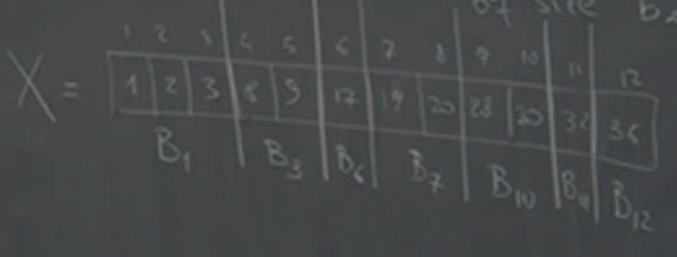
\includegraphics[scale=0.75]{10.png}
\end{center}
For every bucket we have pointers in the index array $I = 1,3,0,0,4,5\ldots$ with the indexes of the beginning and the end of the bucket in $X$. If I want to search for $y$, given that I partitioned the universe I know already the bucket of $y$: it's $B_J$ with $J = \lfloor\frac{y-x_1}{b}\rfloor + 1$, so we do a binary search over $B_J$ looking for $y$. It costs constant, for computing $J$, plus the binary search over $B_J$ which costs $O(\log_2 b)$
\paragraph{Theorem} Time complexity is $O(\log_2 \Delta)$ where $\Delta = \frac{max_{2,\ldots,n} x_i - x_{i-1}}{min_{2,\ldots,n} x_i - x_{i-1}}$, the first time that a complexity depends on the distribution of the data.
\subparagraph{Proof} The maximum is surely larger than the average so $max_{2,\ldots,n} x_i - x_{i-1} \geq \frac{\sum_{i=1}^m x_i - x_{i-1}}{n-1}$, again a telescopic sum, so $= \frac{x_n - x_1}{n-1} \geq \frac{x_n - x_1 + 1}{n} = b$. So $$max_{2,\ldots,n} x_i - x_{i-1} \geq b$$
$$|B_J| \leq \frac{b}{min_{2,\ldots,n} x_i - x_{i-1}} \leq \frac{max_{2,\ldots,n} x_i - x_{i-1}}{min_{2,\ldots,n} x_i - x_{i-1}} = \Delta$$

%Lecture of 12/10
\paragraph{Variable byte econding} Idea is that given a variable $i$ there's a binary representation $B(i)$, for example $i = 2$, then $B(i) = 10$. We use 1 bit out of 8 to make the code prefix free. So $B(i)$ is splitted in blocks of 7 bits, $B(i) = \underline{\textit{000}1101}\:\underline{1001111}$. The most importanti 7 bits become a byte of $\textbf{1}0001101$ and the other $\textbf{0}101111$. Continuation bit is one if the encoding continues and 0 if the encoding ends.\\
Wasteful because we never have the initial byte of the representation (most significal bits) can never be all zero.\\
Not used in practice, lets see how to avoid the waste of space. 1 byte: 128 values ($2^7$), with 2 bytes we have 14 bits and $2^{14}$ values and so on. Using one or two bytes we can encode $2^7 + 2^{14}$ different values. This is done as follows: suppose to have $0\leq i < 2^7 + 2^{14}$. If $i < 2^7 \Rightarrow$ one byte with continuation bit $= 0$. If $2^7 \leq i < 2^7 + 2^{14}$ I encode $i-2^7$ in two bytes. Clearly $0\leq i - 2^7 < 2^{14}$.\\
Reasoning in the same way with 3 bytes we can encode up to $2^7 + 2^{14} + 2^{21}$ different integers.
\paragraph{$(s, c)$ dense codes} Again byte oriented. $s$ stoppers and $c$ continuers.\\
We had every value with last bit $0$ was a stopper, while every value with continuation bit $1$ was a continuer. This means that the values in range $[0, 127]$ were all stoppers, and in range $[128, 255]$ are continuers.\\
We have chosen to have $s$ stoppers and $c$ continuers. We must have $s + c = 256$. With one byte necessarily a stopper, so $s$ possible values. With 2 bytes, first continuer second stopper so total number is $cs$ possible values.\\With three bytes, 2 continuers and last stopper so $c^2 s$ possible values. Using up to three bytes the total number of possible values is $s + cs + c^2s = s(1 + c + c^2)$ which is a geometric progression of ration $c$ $=s\frac{c^3 - 1}{c-2}$. In general using up to $k$ bytes we can encode $s\frac{(c^k - 1)}{c-1}$ different values.\\\\
Suppose we are encoding all positive integers $(\geq 0)$. Given $i$, how many bytes necessary to encode it? I have to find the value $k\:|\:s\frac{c^{k-1} - 1}{c-1}\leq i < s\frac{c^k-1}{c-1}$, cannot be encoded with $k-1$ bytes but can be encoded with $k$ bytes. Found $k$ we can conclude that $i$ will be encoded with $k$ bytes.
\subparagraph{Example} $s+c = 8$ so the combinations are $s, c = 4$, $s = 6, c = 2$, $s = 5, c = 3$.\\
%TODO
I need $k=4$ blocks, with 4 blocks we encode values in $[65, 200]$. 100 is the $100-65 = 35$th value encoded with $k=4$ blocks.
\end{document}